\documentclass[aspectratio=169,12pt,t]{beamer}

% --- Theme: Metropolis (modern, clean) ---
\usetheme[progressbar=frametitle,numbering=fraction,block=fill]{metropolis}

% --- Fira Sans font (install texlive-fonts-extra if missing) ---
\IfFileExists{FiraSans.sty}{\usepackage[sfdefault]{FiraSans}}{}

% --- Light background with warm accent ---
\definecolor{mDarkTeal}{RGB}{35,55,59}
\definecolor{mLightBrown}{RGB}{235,228,216}
\definecolor{mAccent}{RGB}{140,70,20}

\setbeamercolor{normal text}{fg=mDarkTeal,bg=white}
\setbeamercolor{alerted text}{fg=mAccent}
\setbeamercolor{frametitle}{bg=mDarkTeal,fg=white}
\setbeamercolor{progress bar}{fg=mAccent,bg=mLightBrown}
\setbeamercolor{title separator}{fg=mAccent}
\setbeamercolor{progress bar in head/foot}{fg=mAccent,bg=mLightBrown}
\setbeamercolor{progress bar in section page}{fg=mAccent,bg=mLightBrown}

% --- Packages ---
\usepackage[utf8]{inputenc}
\usepackage{amsmath,amssymb,amsthm}
\usepackage{mathrsfs}
\usepackage{tikz}
\usetikzlibrary{arrows.meta,positioning,calc,decorations.pathreplacing,shapes,patterns}
\usepackage{pgfplots}
\pgfplotsset{compat=1.18}

% --- TikZ diagram styles (shared across the series) ---
\tikzset{
  axisln/.style={-{Stealth[length=2.6mm]}, line width=0.8pt, gray!75},
  curveln/.style={line width=1.6pt, line cap=round, line join=round},
  projln/.style={dash pattern=on 2.6pt off 2pt, line width=0.7pt},
  guide/.style={-{Stealth[length=2.6mm,width=2.2mm]}, line width=1.1pt},
}
% point marker with a white halo: \dotpt{color}{(coord)}
\newcommand{\dotpt}[2]{%
  \fill[white] #2 circle (3.6pt);
  \fill[#1] #2 circle (2.4pt);
}
% open point marker: \opendotpt{color}{(coord)}
\newcommand{\opendotpt}[2]{%
  \fill[white] #2 circle (3.6pt);
  \draw[#1, line width=1pt] #2 circle (2.4pt);
}

% --- Semi-transparent white highlight for text on top of background images ---
\usepackage[most]{tcolorbox}

% Inline highlight: \hl{short text}
\newtcbox{\hl}{%
  nobeforeafter, tcbox raise base,
  colback=white, opacityback=0.6,
  colframe=white, opacityframe=0,
  sharp corners, boxsep=2pt, left=3pt, right=3pt, top=2pt, bottom=2pt%
}

% Block highlight: \begin{hlbox} ... \end{hlbox}  (multi-line, paragraphs, itemize)
% Optional argument accepts any tcolorbox key, e.g. [width=0.6\linewidth]
\newtcolorbox{hlbox}[1][]{%
  enhanced, breakable,
  colback=white, opacityback=0.6,
  colframe=white, opacityframe=0,
  boxsep=3pt, left=6pt, right=6pt, top=4pt, bottom=4pt,
  sharp corners,
  {#1}%
}

% --- Custom colors for content types ---
\definecolor{defcolor}{RGB}{25,85,120}
\definecolor{thmcolor}{RGB}{140,35,35}
\definecolor{proofcolor}{RGB}{35,100,50}
\definecolor{excolor}{RGB}{140,75,10}
\definecolor{remcolor}{RGB}{90,90,90}

% --- Beamer blocks for mathematical content types (semi-transparent) ---
\tcbset{hlblockbase/.style={
  enhanced, breakable,
  coltitle=white, fonttitle=\bfseries,
  opacitybacktitle=0.8, opacityback=0.6,
  opacityframe=0,
  sharp corners,
  boxsep=1pt, left=5pt, right=5pt, top=2pt, bottom=2pt,
  toptitle=1pt, bottomtitle=1pt
}}

\newtcolorbox{defblock}[1]{hlblockbase, title={#1},
  colbacktitle=defcolor, colback=defcolor!15, colframe=defcolor}
\newtcolorbox{thmblock}[1]{hlblockbase, title={#1},
  colbacktitle=thmcolor, colback=thmcolor!15, colframe=thmcolor}
\newtcolorbox{proofblock}[1]{hlblockbase, title={#1},
  colbacktitle=proofcolor, colback=proofcolor!15, colframe=proofcolor}
\newtcolorbox{exblock}[1]{hlblockbase, title={#1},
  colbacktitle=excolor, colback=excolor!15, colframe=excolor}
\newtcolorbox{remblock}[1]{hlblockbase, title={#1},
  colbacktitle=remcolor, colback=remcolor!15, colframe=remcolor}

% --- Metadata ---
\title{Chapter 5: Differentiation}
\subtitle{Section: Taylor's Theorem}
\author{Based on Walter Rudin's \emph{Principles of Mathematical Analysis}}
\date{}

\begin{document}

{
\usebackgroundtemplate{%
  
\includegraphics[width=\paperwidth,height=\paperheight,keepaspectratio=false]{chapter_05_bg_00.png}%
}
\begin{frame}[plain]
  \titlepage

  \note{
    Welcome to Chapter 5, Section 6: Taylor's Theorem. This episode is the
    payoff of everything we have built in this chapter. In Section 1 we
    defined the derivative; in Section 2 we proved the mean value theorems;
    and in the previous episode we climbed the tower of higher order
    derivatives: "f" prime, "f" double prime, and so on up to the
    derivative of order "n". Today all of that machinery comes together in
    a single result, Theorem 5.15, known as Taylor's theorem. It says that
    a function with "n" derivatives can be approximated by a polynomial of
    degree "n" minus one, and, crucially, it tells us exactly what the
    error of that approximation looks like. It is one of the most useful
    theorems in all of analysis. Let's dive in.
  }
\end{frame}
}

{
\usebackgroundtemplate{%
  
\includegraphics[width=\paperwidth,height=\paperheight,keepaspectratio=false]{chapter_05_bg_01.png}%
}
\begin{frame}[c]{Outline}
  \begin{center}
    \tableofcontents
  \end{center}

  \note{
    Here is the plan for this episode. We start with motivation: we revisit
    the mean value theorem and see how Taylor's theorem grows out of it as
    a natural upgrade, replacing constants by polynomials. We then
    introduce the star of the show, the Taylor polynomial, and understand
    the sense in which it is the best polynomial approximation to "f" at a
    point. With the polynomial in hand, we state Theorem 5.15, look at its
    special case, and see how it lets us estimate errors in practice. The
    heart of the episode is the proof, a beautiful cascade of mean value
    theorem applications. Finally we summarize and preview the last section
    of this chapter.
  }
\end{frame}

\section{Motivation}

% --- Build 1/3 ---
\begin{frame}{From the Mean Value Theorem to Taylor}
  \begin{hlbox}
  \begin{itemize}
    \item The mean value theorem (5.10), rewritten:
      \[
        f(\beta) = \underbrace{f(\alpha)}_{\text{constant approximation}}
        + \underbrace{f'(x)(\beta - \alpha)}_{\text{exact error term}}
        \qquad \text{for some } x \text{ between } \alpha, \beta
      \]
  \end{itemize}
  \end{hlbox}

  \note{
    Let's start from something we already know. The slide shows the mean
    value theorem, Theorem 5.10, rewritten in a suggestive way: "f" of
    beta equals "f" of alpha, plus "f" prime of "x" times beta minus
    alpha, for some "x" between the two points. The labels under the
    braces spell out the new reading: "f" of alpha is a constant
    approximation to "f" near alpha, and the second term is an exact
    error term, the first derivative at some intermediate point times
    beta minus alpha. A crude approximation, but with a perfectly
    precise error formula. That precision is what we want to keep.
  }
\end{frame}

% --- Build 2/3 ---
\begin{frame}{From the Mean Value Theorem to Taylor}
  \begin{hlbox}
  \begin{itemize}
    \item The mean value theorem (5.10), rewritten:
      \[
        f(\beta) = \underbrace{f(\alpha)}_{\text{constant approximation}}
        + \underbrace{f'(x)(\beta - \alpha)}_{\text{exact error term}}
        \qquad \text{for some } x \text{ between } \alpha, \beta
      \]
    \item With $n$ derivatives available, we can do better:\\
      approximate $f$ by a \alert{polynomial of degree $n-1$} built at $\alpha$
  \end{itemize}
  \end{hlbox}

  \note{
    Now suppose "f" has not just one derivative but "n" of them, as in the
    tower from the previous episode. Then approximating by a constant is
    wasteful; we are ignoring almost everything we know about "f" at
    alpha. The second bullet states the natural upgrade: use all the
    derivatives up to order "n" minus one to build a polynomial of degree
    "n" minus one that imitates "f" near alpha as closely as possible. The
    question is whether we can still say something exact about the error.
  }
\end{frame}

% --- Build 3/3 ---
\begin{frame}{From the Mean Value Theorem to Taylor}
  \begin{hlbox}
  \begin{itemize}
    \item The mean value theorem (5.10), rewritten:
      \[
        f(\beta) = \underbrace{f(\alpha)}_{\text{constant approximation}}
        + \underbrace{f'(x)(\beta - \alpha)}_{\text{exact error term}}
        \qquad \text{for some } x \text{ between } \alpha, \beta
      \]
    \item With $n$ derivatives available, we can do better:\\
      approximate $f$ by a \alert{polynomial of degree $n-1$} built at $\alpha$
    \item \alert{Taylor's theorem:} the error keeps the \emph{same shape} ---
      one $n$th derivative at one unknown point:
      $\dfrac{f^{(n)}(x)}{n!}(\beta-\alpha)^n$
  \end{itemize}
  \end{hlbox}

  \note{
    And here is the remarkable answer, the content of Taylor's theorem.
    When we pass from the constant approximation to the polynomial of
    degree "n" minus one, the error term keeps exactly the same shape as
    in the mean value theorem. It is the derivative of order "n",
    evaluated at a single unknown point "x" between alpha and beta,
    divided by "n" factorial, times beta minus alpha raised to the power
    "n". One derivative, one mystery point, one clean formula. Before we
    make this precise, let's see with our own eyes how good these
    polynomial approximations are.
  }
\end{frame}

\begin{frame}[c]{Taylor Polynomials Hug the Curve}
  \begin{center}
  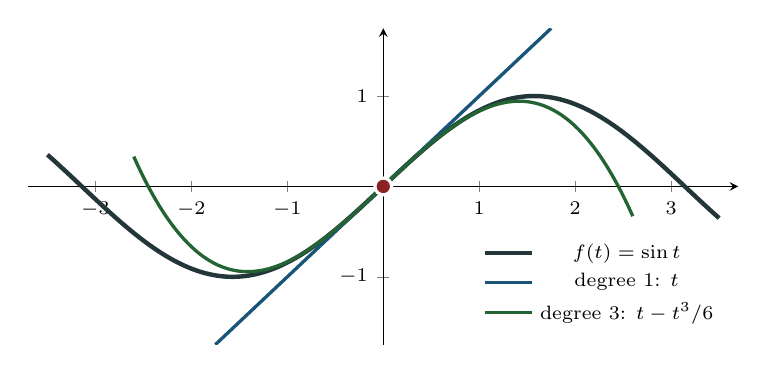
\begin{tikzpicture}
    \begin{axis}[
      width=10.6cm, height=5.6cm,
      axis lines=middle,
      xmin=-3.7, xmax=3.7, ymin=-1.75, ymax=1.75,
      xtick={-3,-2,-1,1,2,3}, ytick={-1,1},
      tick label style={font=\scriptsize},
      legend style={font=\scriptsize, at={(0.985,0.03)}, anchor=south east,
        draw=none, fill=white, fill opacity=0.8, text opacity=1},
    ]
      \addplot[mDarkTeal, line width=1.6pt, domain=-3.5:3.5, samples=160]
        {sin(deg(x))};
      \addlegendentry{$f(t)=\sin t$}
      \addplot[defcolor, line width=1.2pt, domain=-1.75:1.75, samples=2]
        {x};
      \addlegendentry{degree $1$: $t$}
      \addplot[proofcolor, line width=1.2pt, domain=-2.6:2.6, samples=120]
        {x - x^3/6};
      \addlegendentry{degree $3$: $t - t^3/6$}
      \dotpt{thmcolor}{(axis cs:0,0)}
    \end{axis}
  \end{tikzpicture}
  \end{center}

  \vspace{0.2em}
  \begin{center}
    \begin{hlbox}
    Both polynomials are built \alert{only} from derivatives of $f$
    at the red point $\alpha = 0$.
    \end{hlbox}
  \end{center}

  \note{
    Here is the phenomenon in a picture. The dark teal curve is the sine
    function, which we take for granted as in Example 5.6; its rigorous
    treatment comes in Chapter 8. The red dot marks the point alpha equals
    zero, where we collect our information. The blue straight line is the
    degree one approximation, the tangent line: "t" itself. It hugs the
    curve near zero but peels away quickly. The green curve is the degree
    three approximation, "t" minus "t" cubed over six. Look how much
    longer it stays glued to the sine curve, following it well past one on
    each side. Both polynomials were built using only derivatives of "f"
    at the single red point. More derivatives, better approximation, and
    Taylor's theorem will tell us precisely how good. Let's set up the
    exact hypotheses.
  }
\end{frame}
}

{
\usebackgroundtemplate{%
  
\includegraphics[width=\paperwidth,height=\paperheight,keepaspectratio=false]{chapter_05_bg_02.png}%
}
\section{The Taylor Polynomial}

% --- Build 1/2 ---
\begin{frame}{The Setup for Theorem 5.15}
  \begin{defblock}{Standing hypotheses}
    \begin{itemize}
      \item $f$ is a \alert{real} function on $[a,b]$; \ $n$ is a positive integer
      \item $f^{(n-1)}$ is \alert{continuous} on $[a,b]$
      \item $f^{(n)}(t)$ exists for every $t \in (a,b)$
    \end{itemize}
  \end{defblock}

  \note{
    Here are the standing hypotheses; notice that Rudin asks for exactly
    what the proof will need, and not a drop more. First, "f" is a real
    function on the closed interval from "a" to "b", and "n" is a
    positive integer. Second, the derivative of order "n" minus one
    exists and is continuous on the whole closed interval, endpoints
    included. Third, the derivative of order "n" is required to exist
    only at interior points, and nothing is said about its continuity.
    Recall from the previous episode that this already forces all the
    lower floors of the tower of derivatives to behave well. Next we
    introduce the two special points.
  }
\end{frame}

% --- Build 2/2 ---
\begin{frame}{The Setup for Theorem 5.15}
  \begin{defblock}{Standing hypotheses}
    \begin{itemize}
      \item $f$ is a \alert{real} function on $[a,b]$; \ $n$ is a positive integer
      \item $f^{(n-1)}$ is \alert{continuous} on $[a,b]$
      \item $f^{(n)}(t)$ exists for every $t \in (a,b)$
    \end{itemize}
  \end{defblock}

  \begin{defblock}{Two distinct points}
    $\alpha, \beta$ are \alert{distinct} points of $[a,b]$:
    \begin{center}
      $\alpha$ = where we \emph{know} $f$ \ (center of expansion)\\[2pt]
      $\beta$ = where we \emph{want} $f$ \ (target)
    \end{center}
  \end{defblock}

  \note{
    Finally, we fix two distinct points alpha and beta in the interval.
    Think of them as playing different roles. Alpha is the center of
    expansion: the place where we know everything, namely the values of
    "f" and its derivatives up to order "n" minus one. Beta is the target:
    the place where we want to predict the value of "f". Note that the
    theorem does not care which of the two is larger; alpha can lie to the
    left or to the right of beta. With the cast assembled, we can now
    build the polynomial.
  }
\end{frame}

\begin{frame}{The Taylor Polynomial}
  \begin{defblock}{The Taylor polynomial of $f$ at $\alpha$}
    \begin{equation}
      P(t) = \sum_{k=0}^{n-1} \frac{f^{(k)}(\alpha)}{k!}\,(t - \alpha)^k
      \tag{23}
    \end{equation}
  \end{defblock}

  \vspace{0.4em}
  \begin{hlbox}
  Written out:
  \[
    P(t) = f(\alpha) + f'(\alpha)(t-\alpha)
    + \frac{f''(\alpha)}{2!}(t-\alpha)^2 + \cdots
    + \frac{f^{(n-1)}(\alpha)}{(n-1)!}(t-\alpha)^{n-1}
  \]
  \end{hlbox}

  \note{
    Equation 23 defines the Taylor polynomial "P". It is a sum over "k"
    from zero to "n" minus one, and the term of index "k" is the
    derivative of order "k" of "f" at alpha, divided by "k" factorial,
    times "t" minus alpha raised to the power "k". Below the block the sum
    is written out term by term: the constant term is "f" of alpha, the
    linear term is "f" prime of alpha times "t" minus alpha, then the
    second derivative over two factorial times the square, and so on. The
    first two terms alone give the tangent line, so "P" starts from the
    familiar linear approximation and keeps refining it. Notice that "P"
    is a polynomial of degree at most "n" minus one, and it is completely
    determined by data at the single point alpha. Why these particular
    coefficients? The next slide gives the answer.
  }
\end{frame}

\begin{frame}{Why $P$ Is the Right Polynomial}
  \begin{remblock}{$P$ copies all available derivatives of $f$ at $\alpha$}
    \[
      P^{(k)}(\alpha) = f^{(k)}(\alpha)
      \qquad \text{for } k = 0, 1, \dots, n-1
    \]
  \end{remblock}

  \vspace{0.4em}
  \begin{hlbox}
  \textbf{Reason:} differentiating $\dfrac{(t-\alpha)^j}{j!}$ exactly $k$
  times and setting $t = \alpha$ gives $1$ if $j = k$, and $0$ otherwise.
  Each coefficient of $P$ is tuned to match one derivative.
  \end{hlbox}

  \note{
    Here is the sense in which "P" is the best possible choice. The gray
    box says that the derivative of order "k" of "P" at alpha equals the
    derivative of order "k" of "f" at alpha, for every "k" from zero up to
    "n" minus one. In words: "P" has the same value as "f" at alpha, the
    same first derivative, the same second derivative, all the way up to
    order "n" minus one. The reason is the little computation below the
    box. Take a single building block, "t" minus alpha to the power "j"
    over "j" factorial, and differentiate it "k" times at alpha. If "j"
    equals "k" you get exactly one; otherwise you get zero, because either
    a positive power of "t" minus alpha survives, or the term has been
    differentiated away entirely. So each coefficient of "P" is tuned to
    match exactly one derivative of "f", and no coefficient interferes
    with the others. This matching property is precisely what the proof
    will exploit. Now for the theorem itself.
  }
\end{frame}
}

{
\usebackgroundtemplate{%
  
\includegraphics[width=\paperwidth,height=\paperheight,keepaspectratio=false]{chapter_05_bg_03.png}%
}
\section{Taylor's Theorem}

\begin{frame}{Theorem 5.15: Taylor's Theorem}
  \begin{thmblock}{Theorem 5.15 (Taylor)}
    Under the standing hypotheses, there exists a point $x$
    \alert{between $\alpha$ and $\beta$} such that
    \begin{equation}
      f(\beta) = P(\beta) + \frac{f^{(n)}(x)}{n!}\,(\beta - \alpha)^n.
      \tag{24}
    \end{equation}
  \end{thmblock}

  \vspace{0.5em}
  \begin{hlbox}
  \textbf{Key idea:} the value of $f$ at $\beta$ = polynomial prediction
  $+$ an \alert{exact} error term of mean-value type.
  \end{hlbox}

  \note{
    Here it is, Theorem 5.15, Taylor's theorem. Under the hypotheses we
    fixed, there exists a point "x" strictly between alpha and beta such
    that equation 24 holds: "f" of beta equals "P" of beta, the polynomial
    prediction, plus the derivative of order "n" at "x", divided by "n"
    factorial, times beta minus alpha to the power "n". Pause on how
    strong this is. It is not an approximate statement; it is an exact
    identity. All the messiness of the unknown function "f" is compressed
    into the single unknown point "x". We do not know where "x" is, only
    that it lies between alpha and beta, but that is exactly the same kind
    of information the mean value theorem gives. In fact, let's check that
    the mean value theorem is literally the simplest case of this result.
  }
\end{frame}

\begin{frame}{The Case $n = 1$: The Mean Value Theorem}
  \begin{remblock}{Taylor with $n = 1$}
    The sum (23) has the single term $k = 0$, so $P(t) = f(\alpha)$, and
    (24) reads
    \[
      f(\beta) = f(\alpha) + f'(x)(\beta - \alpha).
    \]
    This is exactly the \alert{mean value theorem} (5.10).
  \end{remblock}

  \vspace{0.5em}
  \hl{Taylor's theorem = \emph{the mean value theorem of order $n$}.}

  \note{
    Set "n" equal to one and watch the theorem collapse into an old
    friend. The sum in equation 23 then has only the term with "k" equal
    to zero, so the polynomial "P" is just the constant "f" of alpha. The
    hypotheses ask that "f" itself be continuous on the closed interval
    and differentiable inside, and equation 24 says: "f" of beta equals
    "f" of alpha plus "f" prime of "x" times beta minus alpha. That is
    word for word the mean value theorem, Theorem 5.10, in the rewritten
    form we saw in the motivation. So Taylor's theorem is not some exotic
    new principle; it is the mean value theorem of order "n", and the
    mean value theorem is Taylor's theorem of order one. This also hints
    at the proof strategy: if the case "n" equals one is the mean value
    theorem, perhaps the general case follows by applying the mean value
    theorem "n" times. It does. But first, let's see why the theorem is
    so useful in practice.
  }
\end{frame}

\begin{frame}{What the Theorem Buys Us: Error Estimates}
  \begin{remblock}{From an unknown point to a usable bound}
    If $\bigl|f^{(n)}(t)\bigr| \le M$ for all $t$ between $\alpha$ and
    $\beta$, then (24) gives
    \[
      \bigl|f(\beta) - P(\beta)\bigr|
      \;\le\; \frac{M}{n!}\,\lvert\beta - \alpha\rvert^{n}.
    \]
  \end{remblock}

  \vspace{0.5em}
  \begin{hlbox}
  \begin{itemize}
    \item $f$ can be \alert{computed} to any accuracy from finitely many
      derivatives
    \item $n!$ grows extremely fast --- the bound improves rapidly with $n$
  \end{itemize}
  \end{hlbox}

  \note{
    We never learn where the mystery point "x" is, and remarkably, we
    almost never need to. The gray box shows the standard way the theorem
    is used. Suppose we know a bound: the absolute value of the derivative
    of order "n" is at most "M" everywhere between alpha and beta. Since
    "x" lies in that range, equation 24 immediately gives the estimate on
    the slide: the error of the polynomial approximation is at most "M"
    over "n" factorial, times the distance from alpha to beta raised to
    the power "n". This turns Taylor's theorem into a computational tool.
    As the first bullet says, we can compute values of a complicated
    function to any desired accuracy from finitely many derivatives at
    one point; this is essentially how tables of sines and exponentials
    were computed for centuries. And as the second bullet notes, the "n"
    factorial in the denominator grows extremely fast, so the bounds
    improve dramatically as "n" increases. Now let's prove the theorem.
  }
\end{frame}
}

{
\usebackgroundtemplate{%
  
\includegraphics[width=\paperwidth,height=\paperheight,keepaspectratio=false]{chapter_05_bg_04.png}%
}
\section{Proof of Taylor's Theorem}

\begin{frame}{Proof Strategy}
  \begin{hlbox}
  \textbf{Goal:} find $x$ between $\alpha$ and $\beta$ with
  $f(\beta) = P(\beta) + \dfrac{f^{(n)}(x)}{n!}(\beta-\alpha)^n$.

  \vspace{0.3em}
  \textbf{Approach:}
  \begin{enumerate}
    \item Let $M$ be the number that makes
      $f(\beta) = P(\beta) + M(\beta-\alpha)^n$ true.
      Then show $n!\,M = f^{(n)}(x)$ for some $x$ between $\alpha$ and $\beta$
    \item Build the auxiliary function $g(t) = f(t) - P(t) - M(t-\alpha)^n$
    \item Reduce the goal to: $g^{(n)}(x) = 0$ for some $x$
    \item $g$ vanishes $n$ times over: repeated mean value theorem
      produces such an~$x$
  \end{enumerate}

  \vspace{0.2em}
  \textbf{Technique:} auxiliary function $+$ iterated mean value theorem.
  \end{hlbox}

  \note{
    Before the formal argument, here is the plan of attack, in four steps.
    Step one: instead of hunting for "x" directly, we define "M" to be
    the number that makes the conclusion true by brute force; the actual
    error at beta certainly equals some multiple of beta minus alpha to
    the "n", so we let "M" be that multiple. The whole burden then shifts
    to showing that "n" factorial times "M" is a value of the derivative
    of order "n". Step two: we package everything into one auxiliary
    function "g", the difference between "f" and its polynomial
    prediction, corrected by the "M" term. Step three: the goal becomes
    simply that the derivative of order "n" of "g" vanishes somewhere.
    And step four: the function "g" is designed to vanish so many times
    that repeated applications of the mean value theorem force a zero all
    the way up at the level of the derivative of order "n". This
    two-part trick, an auxiliary function plus an iterated mean value
    theorem, is a pattern worth remembering. Let's carry it out.
  }
\end{frame}

\begin{frame}{Proof of Theorem 5.15 --- Step 1: Define $M$ and $g$}
  \begin{proofblock}{Step 1: Set up}
    Let $M$ be the (unique) number defined by
    \begin{equation}
      f(\beta) = P(\beta) + M(\beta - \alpha)^n
      \tag{25}
    \end{equation}
    and put
    \begin{equation}
      g(t) = f(t) - P(t) - M(t - \alpha)^n \qquad (a \le t \le b).
      \tag{26}
    \end{equation}
  \end{proofblock}

  \vspace{0.4em}
  \hl{\textbf{To show:} $n!\,M = f^{(n)}(x)$ for some $x$ between $\alpha$
  and $\beta$.}

  \note{
    Step one. Equation 25 defines the number "M": since alpha and beta
    are distinct, beta minus alpha to the power "n" is not zero, so there
    is exactly one number "M" making the equation true. "M" is simply the
    actual error of the polynomial approximation at beta, rescaled. At
    this point equation 25 contains no information at all; it is just a
    definition. The content of the theorem is the claim at the bottom of
    the slide: "n" factorial times "M" equals the derivative of order "n"
    of "f" at some point "x" between alpha and beta. If we prove that,
    then substituting back into 25 gives exactly equation 24. Equation 26
    introduces the auxiliary function "g": from "f" we subtract the
    polynomial "P" and the correction term "M" times "t" minus alpha to
    the "n". Note that "g" inherits the regularity of "f": subtracting a
    polynomial changes nothing about differentiability. Now let's see
    what the goal looks like in terms of "g".
  }
\end{frame}

\begin{frame}{Proof of Theorem 5.15 --- Step 2: Reduce to a Zero of $g^{(n)}$}
  \begin{proofblock}{Step 2: Differentiate (26) $n$ times}
    $P$ has degree $\le n-1$, so $P^{(n)} \equiv 0$; \quad
    $\bigl[(t-\alpha)^n\bigr]^{(n)} = n!$
    \begin{equation}
      g^{(n)}(t) = f^{(n)}(t) - n!\,M \qquad (a < t < b).
      \tag{27}
    \end{equation}
  \end{proofblock}

  \vspace{0.4em}
  \begin{hlbox}
  \textbf{New goal:} \alert{$g^{(n)}(x) = 0$} for some $x$ between
  $\alpha$ and $\beta$.\\
  Then (27) gives $n!\,M = f^{(n)}(x)$.
  \end{hlbox}

  \note{
    Step two. Differentiate the definition of "g" a full "n" times. The
    polynomial "P" has degree at most "n" minus one, so after "n"
    differentiations it is wiped out completely. The correction term is
    "M" times "t" minus alpha to the power "n", and differentiating that
    power "n" times leaves the constant "n" factorial. The result is
    equation 27: the derivative of order "n" of "g" equals the derivative
    of order "n" of "f", minus "n" factorial times "M", at every interior
    point. Look what this does for us. If we can find a single point "x"
    between alpha and beta where the derivative of order "n" of "g"
    vanishes, then equation 27 says "n" factorial times "M" equals the
    derivative of order "n" of "f" at "x", which is exactly what we need.
    So the entire theorem now rests on producing one zero of one
    derivative. The function "g" was engineered to make zeros plentiful,
    as we check next.
  }
\end{frame}

\begin{frame}{Proof of Theorem 5.15 --- Step 3: $g$ Vanishes Many Times}
  \begin{proofblock}{Step 3: Zeros of $g$ and its derivatives}
    Since $P^{(k)}(\alpha) = f^{(k)}(\alpha)$ for $k = 0, \dots, n-1$:
    \begin{equation}
      g(\alpha) = g'(\alpha) = \cdots = g^{(n-1)}(\alpha) = 0.
      \tag{28}
    \end{equation}
    Moreover, the choice (25) of $M$ gives \ \alert{$g(\beta) = 0$}.
  \end{proofblock}

  \vspace{0.4em}
  \begin{hlbox}
  $g$ vanishes at \alert{both} $\alpha$ and $\beta$, and its
  first $n-1$ derivatives vanish at $\alpha$.
  \end{hlbox}
  
  \note{
    Step three: let's count the zeros of "g". At the point alpha,
    everything vanishes at once. Indeed, "g" is "f" minus "P" minus the
    correction term. The matching property from earlier says that "P"
    copies the derivatives of "f" at alpha up to order "n" minus one, so
    in the difference they cancel. And the correction term "t" minus
    alpha to the power "n" vanishes to order "n" at alpha: it and its
    first "n" minus one derivatives are all zero there. The result is
    equation 28: "g" and its derivatives up to order "n" minus one all
    vanish at alpha. That is "n" separate pieces of information stacked
    at one point. At the other end, the choice of "M" in equation 25 was
    made precisely so that "g" of beta equals zero; that was the whole
    point of the definition. So "g" vanishes at both endpoints, and its
    derivatives vanish in bulk at alpha. Now the mean value theorem
    takes over.
  }
\end{frame}

% --- Build 1/2 ---
\begin{frame}{Proof of Theorem 5.15 --- Step 4: The Cascade}
  \begin{proofblock}{Step 4: First application of the mean value theorem}
    $g(\alpha) = g(\beta) = 0$
    \ $\Longrightarrow$ \
    $g'(x_1) = 0$ for some $x_1$ between $\alpha$ and $\beta$.
  \end{proofblock}

  \note{
    Step four, the cascade. We begin with the function "g" itself. It
    vanishes at alpha and it vanishes at beta. The mean value theorem,
    applied between these two points, produces a point "x" sub 1 strictly
    between them at which the derivative "g" prime vanishes; in symbols,
    "g" prime of "x" sub 1 equals zero. This is the
    special case of the mean value theorem with equal endpoint values,
    often called Rolle's theorem: between two zeros of a differentiable
    function there is a zero of its derivative. One zero of "g" prime is
    found. But recall from equation 28 that "g" prime also vanishes at
    alpha, and that is exactly what lets us repeat the argument one floor
    up.
  }
\end{frame}

% --- Build 2/2 ---
\begin{frame}{Proof of Theorem 5.15 --- Step 4: The Cascade}
  \begin{proofblock}{Step 4: Iterate, using (28) at each stage}
    $g'(\alpha) = g'(x_1) = 0$
    \ $\Longrightarrow$ \
    $g''(x_2) = 0$ for some $x_2$ between $\alpha$ and $x_1$\\[2pt]
    \dots\ after $n$ steps: \
    \alert{$g^{(n)}(x_n) = 0$} for some $x_n$ between $\alpha$ and
    $x_{n-1}$.
  \end{proofblock}

  \begin{center}
  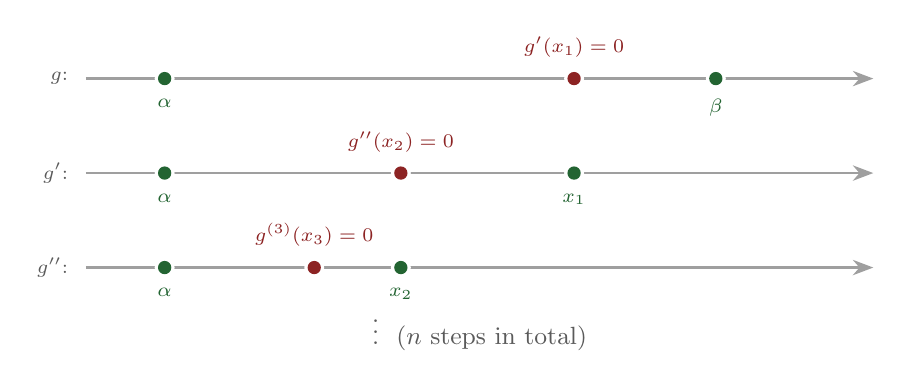
\begin{tikzpicture}[scale=1.0]
    % level 1: g
    \draw[axisln] (0,2.4) -- (10,2.4);
    \dotpt{proofcolor}{(1,2.4)}
    \node[proofcolor, below, font=\scriptsize] at (1,2.26) {$\alpha$};
    \dotpt{proofcolor}{(8,2.4)}
    \node[proofcolor, below, font=\scriptsize] at (8,2.26) {$\beta$};
    \dotpt{thmcolor}{(6.2,2.4)}
    \node[thmcolor, above, font=\scriptsize] at (6.2,2.54) {$g'(x_1)=0$};
    \node[remcolor, font=\scriptsize, left] at (-0.1,2.4) {$g$:};
    % level 2: g'
    \draw[axisln] (0,1.2) -- (10,1.2);
    \dotpt{proofcolor}{(1,1.2)}
    \node[proofcolor, below, font=\scriptsize] at (1,1.06) {$\alpha$};
    \dotpt{proofcolor}{(6.2,1.2)}
    \node[proofcolor, below, font=\scriptsize] at (6.2,1.06) {$x_1$};
    \dotpt{thmcolor}{(4,1.2)}
    \node[thmcolor, above, font=\scriptsize] at (4,1.34) {$g''(x_2)=0$};
    \node[remcolor, font=\scriptsize, left] at (-0.1,1.2) {$g'$:};
    % level 3: g''
    \draw[axisln] (0,0) -- (10,0);
    \dotpt{proofcolor}{(1,0)}
    \node[proofcolor, below, font=\scriptsize] at (1,-0.14) {$\alpha$};
    \dotpt{proofcolor}{(4,0)}
    \node[proofcolor, below, font=\scriptsize] at (4,-0.14) {$x_2$};
    \dotpt{thmcolor}{(2.9,0)}
    \node[thmcolor, above, font=\scriptsize] at (2.9,0.14) {$g^{(3)}(x_3)=0$};
    \node[remcolor, font=\scriptsize, left] at (-0.1,0) {$g''$:};
    % dots
    \node[remcolor, font=\small] at (5,-0.75) {$\vdots$ \ ($n$ steps in total)};
  \end{tikzpicture}
  \end{center}

  \note{
    Now we iterate, and the diagram shows the first three stages. Each
    horizontal line is a copy of the interval, labeled on the left by
    the function it belongs to; green dots mark known zeros, and the
    red dot on each line is the new zero found by the mean value
    theorem. The top line records the step we just took, producing "x"
    sub 1. On the second line, "g" prime vanishes at alpha, by equation
    28, and at "x" sub 1, so between them there is a point "x" sub 2
    where "g" double prime vanishes. The third line repeats the
    argument to produce "x" sub 3. At every stage equation 28 supplies
    the fresh zero at alpha needed to continue. The stockpile of "n"
    zeros at alpha is spent one per stage, so the cascade runs for
    exactly "n" steps, ending with a point "x" sub "n" where the
    derivative of order "n" of "g" vanishes. That is precisely the zero
    we were after.
  }
\end{frame}

\begin{frame}{Proof of Theorem 5.15 --- Conclusion}
  \begin{proofblock}{Conclusion}
    Each $x_k$ lies between $\alpha$ and $x_{k-1}$, hence between
    $\alpha$ and $\beta$. Take $x = x_n$:
    \[
      g^{(n)}(x) = 0
      \ \overset{(27)}{\Longrightarrow}\
      n!\,M = f^{(n)}(x)
      \ \overset{(25)}{\Longrightarrow}\
      \boxed{\,f(\beta) = P(\beta) + \frac{f^{(n)}(x)}{n!}(\beta-\alpha)^n\,}
    \]
  \end{proofblock}

  \vspace{0.4em}
  \hl{This proves (24). \quad $\blacksquare$}

  \note{
    Let's assemble the conclusion. Each point produced by the cascade
    lies between alpha and the previous point, so all of them, in
    particular the last one, lie between alpha and beta. Call that last
    point "x". The cascade tells us the derivative of order "n" of "g"
    vanishes at "x". Feeding this into equation 27, the derivative of
    order "n" of "f" at "x" equals "n" factorial times "M". And
    substituting this value of "M" back into the defining equation 25
    yields the boxed formula: "f" of beta equals "P" of beta plus the
    derivative of order "n" at "x" over "n" factorial, times beta minus
    alpha to the power "n". That is equation 24, and the proof is
    complete. Notice how economical it was: one cleverly chosen auxiliary
    function, and the mean value theorem applied "n" times. Let's step
    back and summarize the episode.
  }
\end{frame}
}

{
\usebackgroundtemplate{%
  
\includegraphics[width=\paperwidth,height=\paperheight,keepaspectratio=false]{chapter_05_bg_05.png}%
}
\section{Summary}

% --- Build 1/3 ---
\begin{frame}{Summary}
  \begin{hlbox}
  \textbf{Key takeaways from this section:}
  \begin{itemize}
    \item \textbf{Theorem 5.15 (Taylor):}
      $f(\beta) = P(\beta) + \frac{f^{(n)}(x)}{n!}(\beta-\alpha)^n$
      for some $x$ between $\alpha$ and $\beta$, where
      $P(t) = \sum_{k=0}^{n-1} \frac{f^{(k)}(\alpha)}{k!}(t-\alpha)^k$
  \end{itemize}
  \end{hlbox}

  \note{
    Let's review what we learned. The headline is Theorem 5.15, Taylor's
    theorem. Under minimal hypotheses, continuity of the derivative of
    order "n" minus one on the closed interval and existence of the
    derivative of order "n" inside, the value of "f" at beta equals the
    Taylor polynomial built at alpha, evaluated at beta, plus an exact
    error term: the derivative of order "n" at some intermediate point
    "x", divided by "n" factorial, times beta minus alpha to the power
    "n". The polynomial copies all the derivatives of "f" at alpha up to
    order "n" minus one, which is what makes it the natural choice.
  }
\end{frame}

% --- Build 2/3 ---
\begin{frame}{Summary}
  \begin{hlbox}
  \textbf{Key takeaways from this section:}
  \begin{itemize}
    \item \textbf{Theorem 5.15 (Taylor):}
      $f(\beta) = P(\beta) + \frac{f^{(n)}(x)}{n!}(\beta-\alpha)^n$
      for some $x$ between $\alpha$ and $\beta$, where
      $P(t) = \sum_{k=0}^{n-1} \frac{f^{(k)}(\alpha)}{k!}(t-\alpha)^k$
    \item \textbf{It generalizes the MVT} ($n=1$), and a bound
      $\lvert f^{(n)}\rvert \le M$ turns it into the error estimate
      $\lvert f(\beta) - P(\beta)\rvert \le \frac{M}{n!}
      \lvert\beta-\alpha\rvert^n$
  \end{itemize}
  \end{hlbox}

  \note{
    Second, perspective and practice. Setting "n" equal to one recovers
    the mean value theorem exactly, so Taylor's theorem deserves to be
    called the mean value theorem of order "n". And although the point
    "x" is unknown, any bound "M" on the derivative of order "n"
    immediately converts equation 24 into a concrete error estimate: the
    polynomial approximates "f" to within "M" over "n" factorial times
    the distance to the power "n". This is the form in which Taylor's
    theorem is used throughout analysis and numerical computation.
  }
\end{frame}

% --- Build 3/3 ---
\begin{frame}{Summary}
  \begin{hlbox}
  \textbf{Key takeaways from this section:}
  \begin{itemize}
    \item \textbf{Theorem 5.15 (Taylor):}
      $f(\beta) = P(\beta) + \frac{f^{(n)}(x)}{n!}(\beta-\alpha)^n$
      for some $x$ between $\alpha$ and $\beta$, where
      $P(t) = \sum_{k=0}^{n-1} \frac{f^{(k)}(\alpha)}{k!}(t-\alpha)^k$
    \item \textbf{It generalizes the MVT} ($n=1$), and a bound
      $\lvert f^{(n)}\rvert \le M$ turns it into the error estimate
      $\lvert f(\beta) - P(\beta)\rvert \le \frac{M}{n!}
      \lvert\beta-\alpha\rvert^n$
    \item \textbf{Proof pattern:} auxiliary function $g = f - P -
      M(t-\alpha)^n$; and a cascade of $n$ mean value theorems
  \end{itemize}

  \vspace{0.4em}
  \textbf{Coming up next:} Differentiation of Vector-Valued Functions ---
  what survives (and what fails!) when $f$ takes values in $\mathbb{R}^k$.
  \end{hlbox}

  \note{
    Third, remember the proof pattern: define the auxiliary function "g"
    by subtracting from "f" both the polynomial and a correction term
    whose coefficient "M" is rigged to create a zero at beta; then a
    cascade of "n" mean value theorem applications pushes that zero up
    the tower of derivatives, one floor at a time. This auxiliary
    function trick appears again and again in analysis, and several
    exercises of this chapter ask you to adapt it. In the next and final
    episode of Chapter 5, we ask what happens to differentiation when
    "f" takes values in the plane or in higher dimensional space. Some
    results survive unchanged, but, surprisingly, the mean value theorem
    and Lopital's rule fail, and we will see explicit counterexamples,
    together with the inequality that comes to the rescue. See you there.
  }
\end{frame}
}

\end{document}
